% !TEX encoding = UTF-8 Unicode
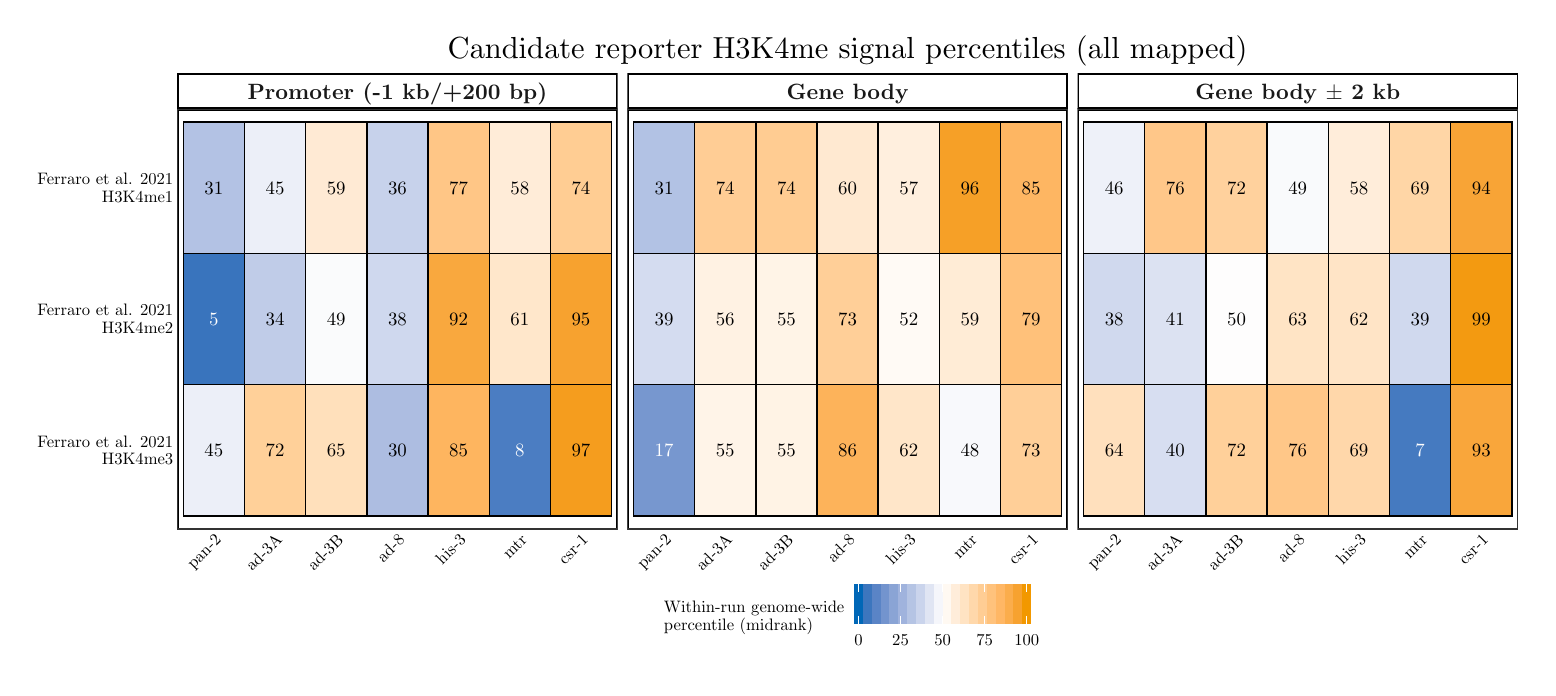
\begin{tikzpicture}[x=1pt,y=1pt]
\definecolor{fillColor}{RGB}{255,255,255}
\path[use as bounding box,fill=fillColor,fill opacity=0.00] (0,0) rectangle (542.02,231.26);
\begin{scope}
\path[clip] (  0.00,  0.00) rectangle (542.02,231.26);
\definecolor{drawColor}{RGB}{255,255,255}
\definecolor{fillColor}{RGB}{255,255,255}

\path[draw=drawColor,line width= 0.7pt,line join=round,line cap=round,fill=fillColor] ( -0.00,  0.00) rectangle (542.02,231.26);
\end{scope}
\begin{scope}
\path[clip] ( 54.02, 50.09) rectangle (213.19,201.87);
\definecolor{drawColor}{RGB}{0,0,0}
\definecolor{fillColor}{RGB}{255,255,255}

\path[draw=drawColor,line width= 1.1pt,line join=round,line cap=round,fill=fillColor] ( 54.02, 50.09) rectangle (213.19,201.87);
\definecolor{fillColor}{RGB}{179,194,228}

\path[draw=drawColor,line width= 0.5pt,fill=fillColor] ( 56.23,149.70) rectangle ( 78.34,197.13);
\definecolor{fillColor}{RGB}{236,239,248}

\path[draw=drawColor,line width= 0.5pt,fill=fillColor] ( 78.34,149.70) rectangle (100.45,197.13);
\definecolor{fillColor}{RGB}{255,234,212}

\path[draw=drawColor,line width= 0.5pt,fill=fillColor] (100.45,149.70) rectangle (122.55,197.13);
\definecolor{fillColor}{RGB}{199,210,235}

\path[draw=drawColor,line width= 0.5pt,fill=fillColor] (122.55,149.70) rectangle (144.66,197.13);
\definecolor{fillColor}{RGB}{255,198,134}

\path[draw=drawColor,line width= 0.5pt,fill=fillColor] (144.66,149.70) rectangle (166.77,197.13);
\definecolor{fillColor}{RGB}{255,236,216}

\path[draw=drawColor,line width= 0.5pt,fill=fillColor] (166.77,149.70) rectangle (188.87,197.13);
\definecolor{fillColor}{RGB}{255,205,147}

\path[draw=drawColor,line width= 0.5pt,fill=fillColor] (188.87,149.70) rectangle (210.98,197.13);
\definecolor{fillColor}{RGB}{57,116,189}

\path[draw=drawColor,line width= 0.5pt,fill=fillColor] ( 56.23,102.27) rectangle ( 78.34,149.70);
\definecolor{fillColor}{RGB}{192,204,232}

\path[draw=drawColor,line width= 0.5pt,fill=fillColor] ( 78.34,102.27) rectangle (100.45,149.70);
\definecolor{fillColor}{RGB}{250,251,252}

\path[draw=drawColor,line width= 0.5pt,fill=fillColor] (100.45,102.27) rectangle (122.55,149.70);
\definecolor{fillColor}{RGB}{207,216,238}

\path[draw=drawColor,line width= 0.5pt,fill=fillColor] (122.55,102.27) rectangle (144.66,149.70);
\definecolor{fillColor}{RGB}{249,168,62}

\path[draw=drawColor,line width= 0.5pt,fill=fillColor] (144.66,102.27) rectangle (166.77,149.70);
\definecolor{fillColor}{RGB}{255,231,203}

\path[draw=drawColor,line width= 0.5pt,fill=fillColor] (166.77,102.27) rectangle (188.87,149.70);
\definecolor{fillColor}{RGB}{247,162,47}

\path[draw=drawColor,line width= 0.5pt,fill=fillColor] (188.87,102.27) rectangle (210.98,149.70);
\definecolor{fillColor}{RGB}{236,239,248}

\path[draw=drawColor,line width= 0.5pt,fill=fillColor] ( 56.23, 54.84) rectangle ( 78.34,102.27);
\definecolor{fillColor}{RGB}{255,208,153}

\path[draw=drawColor,line width= 0.5pt,fill=fillColor] ( 78.34, 54.84) rectangle (100.45,102.27);
\definecolor{fillColor}{RGB}{255,224,187}

\path[draw=drawColor,line width= 0.5pt,fill=fillColor] (100.45, 54.84) rectangle (122.55,102.27);
\definecolor{fillColor}{RGB}{173,189,225}

\path[draw=drawColor,line width= 0.5pt,fill=fillColor] (122.55, 54.84) rectangle (144.66,102.27);
\definecolor{fillColor}{RGB}{254,181,95}

\path[draw=drawColor,line width= 0.5pt,fill=fillColor] (144.66, 54.84) rectangle (166.77,102.27);
\definecolor{fillColor}{RGB}{75,125,194}

\path[draw=drawColor,line width= 0.5pt,fill=fillColor] (166.77, 54.84) rectangle (188.87,102.27);
\definecolor{fillColor}{RGB}{245,157,30}

\path[draw=drawColor,line width= 0.5pt,fill=fillColor] (188.87, 54.84) rectangle (210.98,102.27);

\node[text=drawColor,anchor=base,inner sep=0pt, outer sep=0pt, scale=  0.68] at ( 67.29,171.06) {31};

\node[text=drawColor,anchor=base,inner sep=0pt, outer sep=0pt, scale=  0.68] at ( 89.39,171.06) {45};

\node[text=drawColor,anchor=base,inner sep=0pt, outer sep=0pt, scale=  0.68] at (111.50,171.06) {59};

\node[text=drawColor,anchor=base,inner sep=0pt, outer sep=0pt, scale=  0.68] at (133.61,171.06) {36};

\node[text=drawColor,anchor=base,inner sep=0pt, outer sep=0pt, scale=  0.68] at (155.71,171.06) {77};

\node[text=drawColor,anchor=base,inner sep=0pt, outer sep=0pt, scale=  0.68] at (177.82,171.06) {58};

\node[text=drawColor,anchor=base,inner sep=0pt, outer sep=0pt, scale=  0.68] at (199.93,171.06) {74};
\definecolor{drawColor}{RGB}{255,255,255}

\node[text=drawColor,anchor=base,inner sep=0pt, outer sep=0pt, scale=  0.68] at ( 67.29,123.63) {5};
\definecolor{drawColor}{RGB}{0,0,0}

\node[text=drawColor,anchor=base,inner sep=0pt, outer sep=0pt, scale=  0.68] at ( 89.39,123.63) {34};

\node[text=drawColor,anchor=base,inner sep=0pt, outer sep=0pt, scale=  0.68] at (111.50,123.63) {49};

\node[text=drawColor,anchor=base,inner sep=0pt, outer sep=0pt, scale=  0.68] at (133.61,123.63) {38};

\node[text=drawColor,anchor=base,inner sep=0pt, outer sep=0pt, scale=  0.68] at (155.71,123.63) {92};

\node[text=drawColor,anchor=base,inner sep=0pt, outer sep=0pt, scale=  0.68] at (177.82,123.63) {61};

\node[text=drawColor,anchor=base,inner sep=0pt, outer sep=0pt, scale=  0.68] at (199.93,123.63) {95};

\node[text=drawColor,anchor=base,inner sep=0pt, outer sep=0pt, scale=  0.68] at ( 67.29, 76.20) {45};

\node[text=drawColor,anchor=base,inner sep=0pt, outer sep=0pt, scale=  0.68] at ( 89.39, 76.20) {72};

\node[text=drawColor,anchor=base,inner sep=0pt, outer sep=0pt, scale=  0.68] at (111.50, 76.20) {65};

\node[text=drawColor,anchor=base,inner sep=0pt, outer sep=0pt, scale=  0.68] at (133.61, 76.20) {30};

\node[text=drawColor,anchor=base,inner sep=0pt, outer sep=0pt, scale=  0.68] at (155.71, 76.20) {85};
\definecolor{drawColor}{RGB}{255,255,255}

\node[text=drawColor,anchor=base,inner sep=0pt, outer sep=0pt, scale=  0.68] at (177.82, 76.20) {8};
\definecolor{drawColor}{RGB}{0,0,0}

\node[text=drawColor,anchor=base,inner sep=0pt, outer sep=0pt, scale=  0.68] at (199.93, 76.20) {97};
\definecolor{drawColor}{gray}{0.20}

\path[draw=drawColor,line width= 0.7pt,line join=round,line cap=round] ( 54.02, 50.09) rectangle (213.19,201.87);
\end{scope}
\begin{scope}
\path[clip] (216.69, 50.09) rectangle (375.86,201.87);
\definecolor{drawColor}{RGB}{0,0,0}
\definecolor{fillColor}{RGB}{255,255,255}

\path[draw=drawColor,line width= 1.1pt,line join=round,line cap=round,fill=fillColor] (216.69, 50.09) rectangle (375.86,201.87);
\definecolor{fillColor}{RGB}{178,194,228}

\path[draw=drawColor,line width= 0.5pt,fill=fillColor] (218.90,149.70) rectangle (241.01,197.13);
\definecolor{fillColor}{RGB}{255,205,149}

\path[draw=drawColor,line width= 0.5pt,fill=fillColor] (241.01,149.70) rectangle (263.11,197.13);
\definecolor{fillColor}{RGB}{255,204,146}

\path[draw=drawColor,line width= 0.5pt,fill=fillColor] (263.11,149.70) rectangle (285.22,197.13);
\definecolor{fillColor}{RGB}{255,233,209}

\path[draw=drawColor,line width= 0.5pt,fill=fillColor] (285.22,149.70) rectangle (307.33,197.13);
\definecolor{fillColor}{RGB}{255,239,222}

\path[draw=drawColor,line width= 0.5pt,fill=fillColor] (307.33,149.70) rectangle (329.43,197.13);
\definecolor{fillColor}{RGB}{246,160,39}

\path[draw=drawColor,line width= 0.5pt,fill=fillColor] (329.43,149.70) rectangle (351.54,197.13);
\definecolor{fillColor}{RGB}{254,182,98}

\path[draw=drawColor,line width= 0.5pt,fill=fillColor] (351.54,149.70) rectangle (373.65,197.13);
\definecolor{fillColor}{RGB}{212,220,240}

\path[draw=drawColor,line width= 0.5pt,fill=fillColor] (218.90,102.27) rectangle (241.01,149.70);
\definecolor{fillColor}{RGB}{255,242,227}

\path[draw=drawColor,line width= 0.5pt,fill=fillColor] (241.01,102.27) rectangle (263.11,149.70);
\definecolor{fillColor}{RGB}{255,244,231}

\path[draw=drawColor,line width= 0.5pt,fill=fillColor] (263.11,102.27) rectangle (285.22,149.70);
\definecolor{fillColor}{RGB}{255,207,152}

\path[draw=drawColor,line width= 0.5pt,fill=fillColor] (285.22,102.27) rectangle (307.33,149.70);
\definecolor{fillColor}{RGB}{255,250,245}

\path[draw=drawColor,line width= 0.5pt,fill=fillColor] (307.33,102.27) rectangle (329.43,149.70);
\definecolor{fillColor}{RGB}{255,236,214}

\path[draw=drawColor,line width= 0.5pt,fill=fillColor] (329.43,102.27) rectangle (351.54,149.70);
\definecolor{fillColor}{RGB}{255,193,122}

\path[draw=drawColor,line width= 0.5pt,fill=fillColor] (351.54,102.27) rectangle (373.65,149.70);
\definecolor{fillColor}{RGB}{119,151,207}

\path[draw=drawColor,line width= 0.5pt,fill=fillColor] (218.90, 54.84) rectangle (241.01,102.27);
\definecolor{fillColor}{RGB}{255,244,232}

\path[draw=drawColor,line width= 0.5pt,fill=fillColor] (241.01, 54.84) rectangle (263.11,102.27);
\definecolor{fillColor}{RGB}{255,243,229}

\path[draw=drawColor,line width= 0.5pt,fill=fillColor] (263.11, 54.84) rectangle (285.22,102.27);
\definecolor{fillColor}{RGB}{253,179,90}

\path[draw=drawColor,line width= 0.5pt,fill=fillColor] (285.22, 54.84) rectangle (307.33,102.27);
\definecolor{fillColor}{RGB}{255,230,201}

\path[draw=drawColor,line width= 0.5pt,fill=fillColor] (307.33, 54.84) rectangle (329.43,102.27);
\definecolor{fillColor}{RGB}{248,249,252}

\path[draw=drawColor,line width= 0.5pt,fill=fillColor] (329.43, 54.84) rectangle (351.54,102.27);
\definecolor{fillColor}{RGB}{255,207,152}

\path[draw=drawColor,line width= 0.5pt,fill=fillColor] (351.54, 54.84) rectangle (373.65,102.27);

\node[text=drawColor,anchor=base,inner sep=0pt, outer sep=0pt, scale=  0.68] at (229.95,171.06) {31};

\node[text=drawColor,anchor=base,inner sep=0pt, outer sep=0pt, scale=  0.68] at (252.06,171.06) {74};

\node[text=drawColor,anchor=base,inner sep=0pt, outer sep=0pt, scale=  0.68] at (274.17,171.06) {74};

\node[text=drawColor,anchor=base,inner sep=0pt, outer sep=0pt, scale=  0.68] at (296.27,171.06) {60};

\node[text=drawColor,anchor=base,inner sep=0pt, outer sep=0pt, scale=  0.68] at (318.38,171.06) {57};

\node[text=drawColor,anchor=base,inner sep=0pt, outer sep=0pt, scale=  0.68] at (340.49,171.06) {96};

\node[text=drawColor,anchor=base,inner sep=0pt, outer sep=0pt, scale=  0.68] at (362.59,171.06) {85};

\node[text=drawColor,anchor=base,inner sep=0pt, outer sep=0pt, scale=  0.68] at (229.95,123.63) {39};

\node[text=drawColor,anchor=base,inner sep=0pt, outer sep=0pt, scale=  0.68] at (252.06,123.63) {56};

\node[text=drawColor,anchor=base,inner sep=0pt, outer sep=0pt, scale=  0.68] at (274.17,123.63) {55};

\node[text=drawColor,anchor=base,inner sep=0pt, outer sep=0pt, scale=  0.68] at (296.27,123.63) {73};

\node[text=drawColor,anchor=base,inner sep=0pt, outer sep=0pt, scale=  0.68] at (318.38,123.63) {52};

\node[text=drawColor,anchor=base,inner sep=0pt, outer sep=0pt, scale=  0.68] at (340.49,123.63) {59};

\node[text=drawColor,anchor=base,inner sep=0pt, outer sep=0pt, scale=  0.68] at (362.59,123.63) {79};
\definecolor{drawColor}{RGB}{255,255,255}

\node[text=drawColor,anchor=base,inner sep=0pt, outer sep=0pt, scale=  0.68] at (229.95, 76.20) {17};
\definecolor{drawColor}{RGB}{0,0,0}

\node[text=drawColor,anchor=base,inner sep=0pt, outer sep=0pt, scale=  0.68] at (252.06, 76.20) {55};

\node[text=drawColor,anchor=base,inner sep=0pt, outer sep=0pt, scale=  0.68] at (274.17, 76.20) {55};

\node[text=drawColor,anchor=base,inner sep=0pt, outer sep=0pt, scale=  0.68] at (296.27, 76.20) {86};

\node[text=drawColor,anchor=base,inner sep=0pt, outer sep=0pt, scale=  0.68] at (318.38, 76.20) {62};

\node[text=drawColor,anchor=base,inner sep=0pt, outer sep=0pt, scale=  0.68] at (340.49, 76.20) {48};

\node[text=drawColor,anchor=base,inner sep=0pt, outer sep=0pt, scale=  0.68] at (362.59, 76.20) {73};
\definecolor{drawColor}{gray}{0.20}

\path[draw=drawColor,line width= 0.7pt,line join=round,line cap=round] (216.69, 50.09) rectangle (375.86,201.87);
\end{scope}
\begin{scope}
\path[clip] (379.36, 50.09) rectangle (538.52,201.87);
\definecolor{drawColor}{RGB}{0,0,0}
\definecolor{fillColor}{RGB}{255,255,255}

\path[draw=drawColor,line width= 1.1pt,line join=round,line cap=round,fill=fillColor] (379.36, 50.09) rectangle (538.53,201.87);
\definecolor{fillColor}{RGB}{238,241,249}

\path[draw=drawColor,line width= 0.5pt,fill=fillColor] (381.57,149.70) rectangle (403.67,197.13);
\definecolor{fillColor}{RGB}{255,199,137}

\path[draw=drawColor,line width= 0.5pt,fill=fillColor] (403.67,149.70) rectangle (425.78,197.13);
\definecolor{fillColor}{RGB}{255,209,157}

\path[draw=drawColor,line width= 0.5pt,fill=fillColor] (425.78,149.70) rectangle (447.89,197.13);
\definecolor{fillColor}{RGB}{249,250,252}

\path[draw=drawColor,line width= 0.5pt,fill=fillColor] (447.89,149.70) rectangle (469.99,197.13);
\definecolor{fillColor}{RGB}{255,237,218}

\path[draw=drawColor,line width= 0.5pt,fill=fillColor] (469.99,149.70) rectangle (492.10,197.13);
\definecolor{fillColor}{RGB}{255,214,166}

\path[draw=drawColor,line width= 0.5pt,fill=fillColor] (492.10,149.70) rectangle (514.21,197.13);
\definecolor{fillColor}{RGB}{248,164,54}

\path[draw=drawColor,line width= 0.5pt,fill=fillColor] (514.21,149.70) rectangle (536.31,197.13);
\definecolor{fillColor}{RGB}{208,217,238}

\path[draw=drawColor,line width= 0.5pt,fill=fillColor] (381.57,102.27) rectangle (403.67,149.70);
\definecolor{fillColor}{RGB}{220,226,242}

\path[draw=drawColor,line width= 0.5pt,fill=fillColor] (403.67,102.27) rectangle (425.78,149.70);
\definecolor{fillColor}{RGB}{254,253,253}

\path[draw=drawColor,line width= 0.5pt,fill=fillColor] (425.78,102.27) rectangle (447.89,149.70);
\definecolor{fillColor}{RGB}{255,228,197}

\path[draw=drawColor,line width= 0.5pt,fill=fillColor] (447.89,102.27) rectangle (469.99,149.70);
\definecolor{fillColor}{RGB}{255,228,198}

\path[draw=drawColor,line width= 0.5pt,fill=fillColor] (469.99,102.27) rectangle (492.10,149.70);
\definecolor{fillColor}{RGB}{208,217,238}

\path[draw=drawColor,line width= 0.5pt,fill=fillColor] (492.10,102.27) rectangle (514.21,149.70);
\definecolor{fillColor}{RGB}{243,154,17}

\path[draw=drawColor,line width= 0.5pt,fill=fillColor] (514.21,102.27) rectangle (536.31,149.70);
\definecolor{fillColor}{RGB}{255,224,189}

\path[draw=drawColor,line width= 0.5pt,fill=fillColor] (381.57, 54.84) rectangle (403.67,102.27);
\definecolor{fillColor}{RGB}{215,222,241}

\path[draw=drawColor,line width= 0.5pt,fill=fillColor] (403.67, 54.84) rectangle (425.78,102.27);
\definecolor{fillColor}{RGB}{255,208,154}

\path[draw=drawColor,line width= 0.5pt,fill=fillColor] (425.78, 54.84) rectangle (447.89,102.27);
\definecolor{fillColor}{RGB}{255,199,136}

\path[draw=drawColor,line width= 0.5pt,fill=fillColor] (447.89, 54.84) rectangle (469.99,102.27);
\definecolor{fillColor}{RGB}{255,215,170}

\path[draw=drawColor,line width= 0.5pt,fill=fillColor] (469.99, 54.84) rectangle (492.10,102.27);
\definecolor{fillColor}{RGB}{69,122,192}

\path[draw=drawColor,line width= 0.5pt,fill=fillColor] (492.10, 54.84) rectangle (514.21,102.27);
\definecolor{fillColor}{RGB}{249,166,59}

\path[draw=drawColor,line width= 0.5pt,fill=fillColor] (514.21, 54.84) rectangle (536.31,102.27);

\node[text=drawColor,anchor=base,inner sep=0pt, outer sep=0pt, scale=  0.68] at (392.62,171.06) {46};

\node[text=drawColor,anchor=base,inner sep=0pt, outer sep=0pt, scale=  0.68] at (414.73,171.06) {76};

\node[text=drawColor,anchor=base,inner sep=0pt, outer sep=0pt, scale=  0.68] at (436.83,171.06) {72};

\node[text=drawColor,anchor=base,inner sep=0pt, outer sep=0pt, scale=  0.68] at (458.94,171.06) {49};

\node[text=drawColor,anchor=base,inner sep=0pt, outer sep=0pt, scale=  0.68] at (481.05,171.06) {58};

\node[text=drawColor,anchor=base,inner sep=0pt, outer sep=0pt, scale=  0.68] at (503.15,171.06) {69};

\node[text=drawColor,anchor=base,inner sep=0pt, outer sep=0pt, scale=  0.68] at (525.26,171.06) {94};

\node[text=drawColor,anchor=base,inner sep=0pt, outer sep=0pt, scale=  0.68] at (392.62,123.63) {38};

\node[text=drawColor,anchor=base,inner sep=0pt, outer sep=0pt, scale=  0.68] at (414.73,123.63) {41};

\node[text=drawColor,anchor=base,inner sep=0pt, outer sep=0pt, scale=  0.68] at (436.83,123.63) {50};

\node[text=drawColor,anchor=base,inner sep=0pt, outer sep=0pt, scale=  0.68] at (458.94,123.63) {63};

\node[text=drawColor,anchor=base,inner sep=0pt, outer sep=0pt, scale=  0.68] at (481.05,123.63) {62};

\node[text=drawColor,anchor=base,inner sep=0pt, outer sep=0pt, scale=  0.68] at (503.15,123.63) {39};

\node[text=drawColor,anchor=base,inner sep=0pt, outer sep=0pt, scale=  0.68] at (525.26,123.63) {99};

\node[text=drawColor,anchor=base,inner sep=0pt, outer sep=0pt, scale=  0.68] at (392.62, 76.20) {64};

\node[text=drawColor,anchor=base,inner sep=0pt, outer sep=0pt, scale=  0.68] at (414.73, 76.20) {40};

\node[text=drawColor,anchor=base,inner sep=0pt, outer sep=0pt, scale=  0.68] at (436.83, 76.20) {72};

\node[text=drawColor,anchor=base,inner sep=0pt, outer sep=0pt, scale=  0.68] at (458.94, 76.20) {76};

\node[text=drawColor,anchor=base,inner sep=0pt, outer sep=0pt, scale=  0.68] at (481.05, 76.20) {69};
\definecolor{drawColor}{RGB}{255,255,255}

\node[text=drawColor,anchor=base,inner sep=0pt, outer sep=0pt, scale=  0.68] at (503.15, 76.20) {7};
\definecolor{drawColor}{RGB}{0,0,0}

\node[text=drawColor,anchor=base,inner sep=0pt, outer sep=0pt, scale=  0.68] at (525.26, 76.20) {93};
\definecolor{drawColor}{gray}{0.20}

\path[draw=drawColor,line width= 0.7pt,line join=round,line cap=round] (379.36, 50.09) rectangle (538.53,201.87);
\end{scope}
\begin{scope}
\path[clip] ( 54.02,201.87) rectangle (213.19,214.55);
\definecolor{drawColor}{RGB}{0,0,0}
\definecolor{fillColor}{RGB}{255,255,255}

\path[draw=drawColor,line width= 1.1pt,line join=round,line cap=round,fill=fillColor] ( 54.02,201.87) rectangle (213.19,214.55);
\definecolor{drawColor}{gray}{0.10}

\node[text=drawColor,anchor=base,inner sep=0pt, outer sep=0pt, scale=  0.80] at (133.61,205.45) {\bfseries Promoter (-1 kb/+200 bp)};
\end{scope}
\begin{scope}
\path[clip] (216.69,201.87) rectangle (375.86,214.55);
\definecolor{drawColor}{RGB}{0,0,0}
\definecolor{fillColor}{RGB}{255,255,255}

\path[draw=drawColor,line width= 1.1pt,line join=round,line cap=round,fill=fillColor] (216.69,201.87) rectangle (375.86,214.55);
\definecolor{drawColor}{gray}{0.10}

\node[text=drawColor,anchor=base,inner sep=0pt, outer sep=0pt, scale=  0.80] at (296.27,205.45) {\bfseries Gene body};
\end{scope}
\begin{scope}
\path[clip] (379.36,201.87) rectangle (538.52,214.55);
\definecolor{drawColor}{RGB}{0,0,0}
\definecolor{fillColor}{RGB}{255,255,255}

\path[draw=drawColor,line width= 1.1pt,line join=round,line cap=round,fill=fillColor] (379.36,201.87) rectangle (538.53,214.55);
\definecolor{drawColor}{gray}{0.10}

\node[text=drawColor,anchor=base,inner sep=0pt, outer sep=0pt, scale=  0.80] at (458.94,205.45) {\bfseries Gene body $\pm$ 2 kb};
\end{scope}
\begin{scope}
\path[clip] (  0.00,  0.00) rectangle (542.02,231.26);
\definecolor{drawColor}{RGB}{0,0,0}

\node[text=drawColor,rotate= 45.00,anchor=base east,inner sep=0pt, outer sep=0pt, scale=  0.60] at ( 70.21, 45.77) {pan-2};

\node[text=drawColor,rotate= 45.00,anchor=base east,inner sep=0pt, outer sep=0pt, scale=  0.60] at ( 92.31, 45.77) {ad-3A};

\node[text=drawColor,rotate= 45.00,anchor=base east,inner sep=0pt, outer sep=0pt, scale=  0.60] at (114.42, 45.77) {ad-3B};

\node[text=drawColor,rotate= 45.00,anchor=base east,inner sep=0pt, outer sep=0pt, scale=  0.60] at (136.53, 45.77) {ad-8};

\node[text=drawColor,rotate= 45.00,anchor=base east,inner sep=0pt, outer sep=0pt, scale=  0.60] at (158.63, 45.77) {his-3};

\node[text=drawColor,rotate= 45.00,anchor=base east,inner sep=0pt, outer sep=0pt, scale=  0.60] at (180.74, 45.77) {mtr};

\node[text=drawColor,rotate= 45.00,anchor=base east,inner sep=0pt, outer sep=0pt, scale=  0.60] at (202.85, 45.77) {csr-1};
\end{scope}
\begin{scope}
\path[clip] (  0.00,  0.00) rectangle (542.02,231.26);
\definecolor{drawColor}{RGB}{0,0,0}

\node[text=drawColor,rotate= 45.00,anchor=base east,inner sep=0pt, outer sep=0pt, scale=  0.60] at (232.88, 45.77) {pan-2};

\node[text=drawColor,rotate= 45.00,anchor=base east,inner sep=0pt, outer sep=0pt, scale=  0.60] at (254.98, 45.77) {ad-3A};

\node[text=drawColor,rotate= 45.00,anchor=base east,inner sep=0pt, outer sep=0pt, scale=  0.60] at (277.09, 45.77) {ad-3B};

\node[text=drawColor,rotate= 45.00,anchor=base east,inner sep=0pt, outer sep=0pt, scale=  0.60] at (299.20, 45.77) {ad-8};

\node[text=drawColor,rotate= 45.00,anchor=base east,inner sep=0pt, outer sep=0pt, scale=  0.60] at (321.30, 45.77) {his-3};

\node[text=drawColor,rotate= 45.00,anchor=base east,inner sep=0pt, outer sep=0pt, scale=  0.60] at (343.41, 45.77) {mtr};

\node[text=drawColor,rotate= 45.00,anchor=base east,inner sep=0pt, outer sep=0pt, scale=  0.60] at (365.52, 45.77) {csr-1};
\end{scope}
\begin{scope}
\path[clip] (  0.00,  0.00) rectangle (542.02,231.26);
\definecolor{drawColor}{RGB}{0,0,0}

\node[text=drawColor,rotate= 45.00,anchor=base east,inner sep=0pt, outer sep=0pt, scale=  0.60] at (395.54, 45.77) {pan-2};

\node[text=drawColor,rotate= 45.00,anchor=base east,inner sep=0pt, outer sep=0pt, scale=  0.60] at (417.65, 45.77) {ad-3A};

\node[text=drawColor,rotate= 45.00,anchor=base east,inner sep=0pt, outer sep=0pt, scale=  0.60] at (439.76, 45.77) {ad-3B};

\node[text=drawColor,rotate= 45.00,anchor=base east,inner sep=0pt, outer sep=0pt, scale=  0.60] at (461.86, 45.77) {ad-8};

\node[text=drawColor,rotate= 45.00,anchor=base east,inner sep=0pt, outer sep=0pt, scale=  0.60] at (483.97, 45.77) {his-3};

\node[text=drawColor,rotate= 45.00,anchor=base east,inner sep=0pt, outer sep=0pt, scale=  0.60] at (506.08, 45.77) {mtr};

\node[text=drawColor,rotate= 45.00,anchor=base east,inner sep=0pt, outer sep=0pt, scale=  0.60] at (528.18, 45.77) {csr-1};
\end{scope}
\begin{scope}
\path[clip] (  0.00,  0.00) rectangle (542.02,231.26);
\definecolor{drawColor}{RGB}{0,0,0}

\node[text=drawColor,anchor=base east,inner sep=0pt, outer sep=0pt, scale=  0.60] at ( 52.62, 79.73) {Ferraro et al. 2021};

\node[text=drawColor,anchor=base east,inner sep=0pt, outer sep=0pt, scale=  0.60] at ( 52.62, 73.25) {H3K4me3};

\node[text=drawColor,anchor=base east,inner sep=0pt, outer sep=0pt, scale=  0.60] at ( 52.62,127.16) {Ferraro et al. 2021};

\node[text=drawColor,anchor=base east,inner sep=0pt, outer sep=0pt, scale=  0.60] at ( 52.62,120.68) {H3K4me2};

\node[text=drawColor,anchor=base east,inner sep=0pt, outer sep=0pt, scale=  0.60] at ( 52.62,174.59) {Ferraro et al. 2021};

\node[text=drawColor,anchor=base east,inner sep=0pt, outer sep=0pt, scale=  0.60] at ( 52.62,168.11) {H3K4me1};
\end{scope}
\begin{scope}
\path[clip] (  0.00,  0.00) rectangle (542.02,231.26);
\definecolor{fillColor}{RGB}{255,255,255}

\path[fill=fillColor] (226.43,  3.50) rectangle (366.12, 33.75);
\end{scope}
\begin{scope}
\path[clip] (  0.00,  0.00) rectangle (542.02,231.26);
\definecolor{drawColor}{RGB}{0,0,0}

\node[text=drawColor,anchor=base west,inner sep=0pt, outer sep=0pt, scale=  0.60] at (229.93, 19.80) {Within-run genome-wide};

\node[text=drawColor,anchor=base west,inner sep=0pt, outer sep=0pt, scale=  0.60] at (229.93, 13.32) {percentile (midrank)};
\end{scope}
\begin{scope}
\path[clip] (  0.00,  0.00) rectangle (542.02,231.26);
\definecolor{fillColor}{RGB}{0,103,183}

\path[fill=fillColor] (298.60, 15.80) rectangle (301.80, 30.25);
\definecolor{fillColor}{RGB}{60,118,190}

\path[fill=fillColor] (301.80, 15.80) rectangle (305.00, 30.25);
\definecolor{fillColor}{RGB}{90,132,198}

\path[fill=fillColor] (305.00, 15.80) rectangle (308.20, 30.25);
\definecolor{fillColor}{RGB}{115,148,206}

\path[fill=fillColor] (308.20, 15.80) rectangle (311.40, 30.25);
\definecolor{fillColor}{RGB}{138,164,213}

\path[fill=fillColor] (311.40, 15.80) rectangle (314.60, 30.25);
\definecolor{fillColor}{RGB}{160,179,221}

\path[fill=fillColor] (314.60, 15.80) rectangle (317.80, 30.25);
\definecolor{fillColor}{RGB}{181,196,228}

\path[fill=fillColor] (317.80, 15.80) rectangle (321.00, 30.25);
\definecolor{fillColor}{RGB}{202,212,236}

\path[fill=fillColor] (321.00, 15.80) rectangle (324.21, 30.25);
\definecolor{fillColor}{RGB}{224,229,243}

\path[fill=fillColor] (324.21, 15.80) rectangle (327.41, 30.25);
\definecolor{fillColor}{RGB}{245,246,251}

\path[fill=fillColor] (327.41, 15.80) rectangle (330.61, 30.25);
\definecolor{fillColor}{RGB}{255,249,242}

\path[fill=fillColor] (330.61, 15.80) rectangle (333.81, 30.25);
\definecolor{fillColor}{RGB}{255,237,218}

\path[fill=fillColor] (333.81, 15.80) rectangle (337.01, 30.25);
\definecolor{fillColor}{RGB}{255,227,195}

\path[fill=fillColor] (337.01, 15.80) rectangle (340.21, 30.25);
\definecolor{fillColor}{RGB}{255,216,171}

\path[fill=fillColor] (340.21, 15.80) rectangle (343.41, 30.25);
\definecolor{fillColor}{RGB}{255,205,148}

\path[fill=fillColor] (343.41, 15.80) rectangle (346.61, 30.25);
\definecolor{fillColor}{RGB}{255,194,124}

\path[fill=fillColor] (346.61, 15.80) rectangle (349.81, 30.25);
\definecolor{fillColor}{RGB}{255,183,101}

\path[fill=fillColor] (349.81, 15.80) rectangle (353.01, 30.25);
\definecolor{fillColor}{RGB}{251,173,76}

\path[fill=fillColor] (353.01, 15.80) rectangle (356.21, 30.25);
\definecolor{fillColor}{RGB}{247,162,48}

\path[fill=fillColor] (356.21, 15.80) rectangle (359.42, 30.25);
\definecolor{fillColor}{RGB}{242,152,0}

\path[fill=fillColor] (359.42, 15.80) rectangle (362.62, 30.25);
\end{scope}
\begin{scope}
\path[clip] (  0.00,  0.00) rectangle (542.02,231.26);
\definecolor{drawColor}{RGB}{255,255,255}

\path[draw=drawColor,line width= 0.4pt,line join=round] (300.20, 18.69) --
	(300.20, 15.80);

\path[draw=drawColor,line width= 0.4pt,line join=round] (315.40, 18.69) --
	(315.40, 15.80);

\path[draw=drawColor,line width= 0.4pt,line join=round] (330.61, 18.69) --
	(330.61, 15.80);

\path[draw=drawColor,line width= 0.4pt,line join=round] (345.81, 18.69) --
	(345.81, 15.80);

\path[draw=drawColor,line width= 0.4pt,line join=round] (361.02, 18.69) --
	(361.02, 15.80);

\path[draw=drawColor,line width= 0.4pt,line join=round] (300.20, 27.36) --
	(300.20, 30.25);

\path[draw=drawColor,line width= 0.4pt,line join=round] (315.40, 27.36) --
	(315.40, 30.25);

\path[draw=drawColor,line width= 0.4pt,line join=round] (330.61, 27.36) --
	(330.61, 30.25);

\path[draw=drawColor,line width= 0.4pt,line join=round] (345.81, 27.36) --
	(345.81, 30.25);

\path[draw=drawColor,line width= 0.4pt,line join=round] (361.02, 27.36) --
	(361.02, 30.25);
\end{scope}
\begin{scope}
\path[clip] (  0.00,  0.00) rectangle (542.02,231.26);
\definecolor{drawColor}{RGB}{0,0,0}

\node[text=drawColor,anchor=base,inner sep=0pt, outer sep=0pt, scale=  0.60] at (300.20,  8.17) {0};

\node[text=drawColor,anchor=base,inner sep=0pt, outer sep=0pt, scale=  0.60] at (315.40,  8.17) {25};

\node[text=drawColor,anchor=base,inner sep=0pt, outer sep=0pt, scale=  0.60] at (330.61,  8.17) {50};

\node[text=drawColor,anchor=base,inner sep=0pt, outer sep=0pt, scale=  0.60] at (345.81,  8.17) {75};

\node[text=drawColor,anchor=base,inner sep=0pt, outer sep=0pt, scale=  0.60] at (361.02,  8.17) {100};
\end{scope}
\begin{scope}
\path[clip] (  0.00,  0.00) rectangle (542.02,231.26);
\definecolor{drawColor}{RGB}{0,0,0}

\node[text=drawColor,anchor=base,inner sep=0pt, outer sep=0pt, scale=  1.10] at (296.27,220.19) {Candidate reporter H3K4me signal percentiles (all mapped)};
\end{scope}
\end{tikzpicture}
